\documentclass{article}
\usepackage[a4paper, left=1.5cm, right=1.5cm, top=1cm, bottom=2cm]{geometry}

\usepackage{boldline}
\usepackage{tikz,tcolorbox}
\usepackage{amsmath}
\usepackage[table,xcdraw]{xcolor}
\usepackage{listings}
\usepackage{array,multirow} % For customizing tables
\usepackage{booktabs} % For better horizontal lines
\usepackage{makecell}
\setlength{\parindent}{0pt}
\usepackage{siunitx}
\usepackage{tkz-tab}
\usepackage{amssymb}
\usepackage{amsmath}
\usepackage{enumitem}

\usepackage{caption}
\usepackage{float}


\newcommand{\exer}[1]{
  \section*{Exercice #1}
  \vspace{-0.5cm}
  \noindent\rule{\textwidth}{0.5pt}%
}

\newcommand{\tit}[1]{
\begin{center}
    \Large{\textbf{{#1}}}
\end{center}
}

\definecolor{commentgray}{HTML}{676160}
\definecolor{messagegreen}{HTML}{17B867}
\definecolor{myblue}{HTML}{10C2C4}

\tcbuselibrary{skins, breakable, theorems}
\usepackage{booktabs} 

\newtcolorbox{prettyBox}[2]{
  enhanced,
  colback=white!90!#2,   % Background color based on the second parameter (color)
  colframe=#2!60!black,  % Frame color based on the second parameter (color)
  coltitle=white,        % Title color (white)
  fonttitle=\bfseries\Large,
  title=#1,              % Title from the first parameter
  boxrule=1mm,
  arc=0.5mm,
  drop shadow=#2!35!gray, % Drop shadow color based on the second parameter (color)
}



\lstdefinestyle{cmd}{
 basicstyle=\ttfamily,
 backgroundcolor=\color{lightgray!20},
 frame=single
}

\lstdefinestyle{pythonstyle}{
    language=python,                    % Language set to Python
    basicstyle=\ttfamily\footnotesize,   % Change basic font size
    keywordstyle=\color{blue}\bfseries, % Different keyword style
    stringstyle=\color{red},         % Different string color
    commentstyle=\color{green!60!black}\itshape, % Adjust comment color
    numbers=left,                       % Line numbers on the left
    numberstyle=\tiny\color{gray},      % Smaller number font and color
    stepnumber=1,                       % Number each line
    frame=single,                       % Single frame around code
    tabsize=4,                          % Adjust tab size
    showstringspaces=false,             % Do not show spaces in strings
    captionpos=b,% Position of caption
    breaklines=true,
    inputencoding=utf8
}




\begin{document}
\tit{TD N\(^{\boldsymbol{\circ}}\)\hspace{0.1cm}4}

\vspace{0.35cm}

\begin{prettyBox}{K-NN}{myblue}
    K-NN est un algorithme supervisé qui peut être utilisé pour la classification et la régression. Il prend comme
    paramètre $K$, le nombre de voisins les plus proches.
\end{prettyBox}


\vspace{0.15cm}

\begin{prettyBox}{K-NN Algo}{myblue}
    \begin{enumerate}
        \setlength{\itemsep}{0pt}
        \item Choisir le nombre \(K\) en utilisant l'heuristique : $K \approx \sqrt{N} \quad \text{et } K \text{ est impair}$
            \begin{itemize}
                \setlength{\itemsep}{0pt}
                \item $N$ est le nombre d'instances.
                \item On prend $K$ impair pour éviter une égalité dans le vote (pour la classification).
            \end{itemize}
        \item Calculer la distance entre $X_{\text{test}}$ et tous les points du dataset.
        \item Donner pour chaque point un rang en indexant de la plus petite distance à la plus grande (si même distance, donner le même rang).
        \item Prendre les $K$ plus proches voisins.
        \item Si classification, faire un vote de majorité.
        \item Si régression, faire la moyenne entre les labels des voisins.
    \end{enumerate}
\end{prettyBox}

\vspace{0.25cm}

\begin{prettyBox}{C4.5}{myblue}
    C4.5 est un algorithme supervisé qui génère un arbre de décision utilisé pour 
    la classification. Il divise selon le gain\_ratio.
\end{prettyBox}

\vspace{0.15cm}

\begin{prettyBox}{Entropy $H(Y)$}{myblue}
    L'entropie $H(Y)$ représente le degré de désordre, à quel point les labels sont mélangés. Plus elle est élevée,
    plus il y a un mélange :
    \[ H(Y) = - \sum_{y \in Y} P(y) \cdot \log_2(P(y)) \]
    \begin{itemize}
        \setlength{\itemsep}{0pt}
        \item $y$ représente une classe.
        \item $Y$ représente toutes les classes.
    \end{itemize}
\end{prettyBox}


\vspace{0.15cm}


\begin{prettyBox}{Entropy $H(Y \mid X_i)$}{myblue}
    L'entropie $H(Y)$ représente le désordre restant après avoir utilisé une information (attribut $X_i$) : 
    \[ H(Y \mid X_i) = \sum_{x \in X_i} \dfrac{|D_{x}|}{|D|} \cdot  \left[-\sum_{y \in Y} \dfrac{|D_{x , y}|}{|D_{x}|} \cdot \log_2\left( \dfrac{|D_{x , y}|}{|D_{x}|} \right) \right] \]
    \begin{itemize}
        \setlength{\itemsep}{0pt}
        \item $x$ une valeur de l'attribut $X_i$.
        \item $X_i$ un attribut du data set.
        \item $y$ représente une classe.
        \item $Y$ représente toutes les classes.
        \item $|D|$ est le nombre d'instances.
        \item $|D_x|$ est le nombre d'instances avec $x$.
        \item $|D_{x , y}|$ est le nombre d'instances avec $x$ et $y$.
    \end{itemize}
\end{prettyBox}

\newpage


\begin{prettyBox}{gain($X_i$)}{myblue}
    Mesure combien un attribut ($X_i$) aide à réduire l'incertitude (l'entropie) dans la classification des données :
    \[
        \text{gain}(X_i) = H(Y) - H(Y \mid X_i)
    \]
\end{prettyBox}

\vspace{0.35cm}


\begin{prettyBox}{split\_info($X_i$)}{myblue}
    Une métrique qui mesure l'information potentielle générée en divisant le data set en branche basées sur un attribut ($X_i$) :

    \[ \text{split\_info} (X_i) = -\sum_{x \in X_i} \dfrac{|D_{x}|}{|D|} \cdot \log_2\left( \dfrac{|D_{x}|}{|D|} \right)  \]
\end{prettyBox}

\vspace{0.35cm}

\begin{prettyBox}{gain\_ratio($X_i$)}{myblue}
    Représente l'efficacité d'un critère, en équilibrant l'information gagnée par rapport à la complexité (le nombre de branches) qu'il crée :
    \[
        \text{gain\_ratio}(X_i) = \dfrac{\text{gain}(X_i)}{\text{split\_info}(X_i)}
    \]
\end{prettyBox}

\vspace{0.35cm}

\begin{prettyBox}{C4.5 Algo}{myblue}
    \begin{enumerate}
        \setlength{\itemsep}{0pt}
        \item Calcule l'entropie du label $H(Y)$.
        \item Calcule le gain de tous les attributs $\text{gain}(X)$.
        \item Calcule le split\_info de tous les attributs $\text{split\_info}(X)$.
        \item Calcule le gain\_ratio de tous les attributs $\text{gain\_ratio}(X)$.
        \item Prendre le gain\_ratio le plus grand et diviser le dataset par rapport à l'attribut.
        \item Si aucune classe n'est mélangée, l'arbre de décision est fini.
        \item Sinon, répéter le même traitement pour le sous-ensemble de données.
    \end{enumerate}
\end{prettyBox}

\newpage

\exer{1}

\vspace{0.25cm}

\begin{table}[h]
\centering

\renewcommand{\arraystretch}{1.75} 
\setlength{\tabcolsep}{12pt}      

\begin{tabular}{|c|c|c|c|c|c|} 

\hline
\textbf{Day}  & \textbf{Outlook}  & \textbf{Temperature} & \textbf{Humidity} & \textbf{Wind} & \textbf{PlayTennis?} \\ \hline
1& Sunny& Hot& High &Light & No \\ \hline
2& Sunny &Hot &High &Strong& No \\ \hline
3 &Overcast &Hot &High &Light &Yes \\ \hline
4 &Rain &Mild &High &Light &Yes \\ \hline
5 &Rain &Cool &Normal &Light &Yes \\ \hline
6 &Rain &Cool &Normal &Strong &No \\ \hline
7 &Overcast &Cool &Normal &Strong &Yes \\ \hline
8 &Sunny &Mild &High &Light &No \\ \hline
9 &Sunny &Cool &Normal &Light &Yes \\ \hline
10 &Rain &Mild &Normal &Light &Yes \\ \hline
11 &Sunny &Mild &Normal &Strong &Yes\\ \hline
12 &Overcast &Mild &High &Strong &Yes \\ \hline
13 &Overcast& Hot& Normal &Light& Yes\\ \hline
14 &Rain &Mild &High& Strong& No \\ \hline
\end{tabular}
\end{table}

Utilisez le classifieur Naïve Bayes pour prédire si la personne jouera au tennis étant donné
les nouvelles conditions suivantes : $X_{\text{test}}$ = (sunny, cool, high, light) 

\vspace{0.75cm}
Calcule des probabilites priorie :
\[P(\text{Yes}) = \dfrac{9}{14} \quad , \quad P(\text{No}) = \dfrac{5}{14}\]


\vspace{0.75cm}
Calcule des probabilites conditionelle :

{\footnotesize
\begin{align*}
    P(X_{\text{test}} \mid Y = \text{Yes}) &= P(x_1 = \text{sunny} \mid Y =\text{Yes}) \cdot P(x_2 = \text{cool} \mid Y =\text{Yes}) \cdot P(x_3 = \text{high} \mid Y =\text{Yes}) \cdot P(x_4 = \text{light} \mid Y =\text{Yes})  \\[0.15cm] 
                                           & = \dfrac{2}{9} \cdot \dfrac{3}{9} \cdot \dfrac{3}{9} \cdot \dfrac{6}{9} \\[0.15cm]
                                           & = \dfrac{4}{243}
\end{align*}
}

\vspace{0.25cm}

{\footnotesize
\begin{align*}
    P(X_{\text{test}} \mid Y = \text{No}) &= P(x_1 = \text{sunny} \mid Y =\text{No}) \cdot P(x_2 = \text{cool} \mid Y =\text{No}) \cdot P(x_3 = \text{high} \mid Y =\text{No}) \cdot P(x_4 = \text{light} \mid Y =\text{No})  \\[0.15cm] 
                                           & = \dfrac{3}{5} \cdot \dfrac{1}{5} \cdot \dfrac{4}{5} \cdot \dfrac{2}{5} \\[0.15cm]
                                           & = \dfrac{24}{625}
\end{align*}
}



\vspace{0.75cm}
Calcule des numerateurs :

\begin{align*}
    &\text{Numerateur(Yes)} = P ( X_{\text{test}}  \mid Y = \text{Oui})\cdot P(\text{Yes}) = \dfrac{4}{243} \cdot \dfrac{9}{14} = 0.010\\[0.1cm]
    &\text{Numerateur(No)} = P ( X_{\text{test}} \mid Y = \text{No})\cdot P(\text{No}) = \dfrac{24}{625} \cdot \dfrac{5}{14} = 0.013
\end{align*}

\vspace{0.25cm}

Puisque Numerateur(No) = 0.013 $>$ Numerateur(Yes) = 0.010 le classifieur Naïve Bayes prédit la classe No.\\[0.1cm]
\textbf{Conclusion} : Selon les conditions de test ($X_{\text{text}}$ = (sunny , cool , high , light)) l'algorithme prédit que la personne ne jouera pas au tennis.\\[0.15cm]

\vspace{0.1cm}
Proposer une mesure de similarité entre les instances :\\[0.15cm]
On va utiliser \textbf{la distance euclidienne} mais avant ca on doit transformer les string en chiffre avec \textbf{label encoding} :


\begin{table}[h]
\centering

\renewcommand{\arraystretch}{1.25} 
\setlength{\tabcolsep}{12pt}      

\begin{tabular}{|c|c|c|c|c|c|} 

\hline
\textbf{Day}  & \textbf{Outlook}  & \textbf{Temperature} & \textbf{Humidity} & \textbf{Wind} & \textbf{PlayTennis?} \\ \hline
1& 1 & 1& 1 & 1 & No \\ \hline
2& 1 &1 &1 &2& No \\ \hline
3 &2 &1 &1 &1 &Yes \\ \hline
4 &3 &2 &1 &1 &Yes \\ \hline
5 &3 &3 &2 &1 &Yes \\ \hline
6 &3 &3 &2 &2 &No \\ \hline
7 &2 &3 &2 &2 &Yes \\ \hline
8 &1 &2 &1 &1 &No \\ \hline
9 &1 &3 &2 &1 &Yes \\ \hline
10 &3 &2 &2 &1 &Yes \\ \hline
11 &1 &2 &2 &2 &Yes\\ \hline
12 &2 &2 &1 &2 &Yes \\ \hline
13 &2 & 1& 2 &1& Yes\\ \hline
14 &3 &2 &1& 2& No \\ \hline
\end{tabular}
\end{table}

Appliquer l’algorithme K-NN :\\[0.1cm]
Pour choisir \(K\) on utilisera heuristique \(K \approx \sqrt{N}\) :
\[ \sqrt{N} = \sqrt{14}  = 3.74 \Rightarrow K = 3\]

On calcule les distances et rangs de tout les points avec $X_{\text{text}} = (1,3,1,1) $
\begin{table}[h]
\centering

\renewcommand{\arraystretch}{1.25} 
\setlength{\tabcolsep}{8pt}      

\begin{tabular}{|c|c|c|c|c|c|c|} 

\hline
\textbf{Outlook}  & \textbf{Temp} & \textbf{Humidity} & \textbf{Wind} & \textbf{Play?} & \textbf{Distance} & \textbf{Rang} \\ \hline
1 & 1& 1 & 1 & No &  {\scriptsize $\sqrt{(1-1)^2 + (3-1)^2 + (1-1)^2 + (1-1)^2 }$ = 2 } & 3\\ \hline
1 &1 &1 &2& No &  {\scriptsize $\sqrt{(1-1)^2 + (3-1)^2 + (1-1)^2 + (1-2)^2 }$ = 2.23 }& 4 \\ \hline
2 &1 &1 &1 &Yes &  {\scriptsize $\sqrt{(1-2)^2 + (3-1)^2 + (1-1)^2 + (1-1)^2 }$ = 2.23 } & 4 \\ \hline
3 &2 &1 &1 &Yes &  {\scriptsize $\sqrt{(1-3)^2 + (3-2)^2 + (1-1)^2 + (1-1)^2 }$ = 2.23 } & 4 \\ \hline
3 &3 &2 &1 &Yes &  {\scriptsize $\sqrt{(1-3)^2 + (3-3)^2 + (1-2)^2 + (1-1)^2 }$ = 2.23 } & 4 \\ \hline
3 &3 &2 &2 &No &  {\scriptsize $\sqrt{(1-3)^2 + (3-3)^2 + (1-2)^2 + (1-2)^2 }$ = 2.44 } & 5 \\ \hline
 2 &3 &2 &2 &Yes &  {\scriptsize $\sqrt{(1-2)^2 + (3-3)^2 + (1-2)^2 + (1-2)^2 }$ = 1.73 } & 2 \\ \hline
 1 &2 &1 &1 &No &  {\scriptsize $\sqrt{(1-1)^2 + (3-2)^2 + (1-1)^2 + (1-1)^2 }$ = 1 } & 1 \\ \hline
 1 &3 &2 &1 &Yes &  {\scriptsize $\sqrt{(1-1)^2 + (3-3)^2 + (1-2)^2 + (1-1)^2 }$ = 1 } & 1 \\ \hline
 3 &2 &2 &1 &Yes &  {\scriptsize $\sqrt{(1-3)^2 + (3-2)^2 + (1-2)^2 + (1-1)^2 }$ = 2.44 } & 5 \\ \hline
 1 &2 &2 &2 &Yes &  {\scriptsize $\sqrt{(1-1)^2 + (3-2)^2 + (1-2)^2 + (1-2)^2 }$ = 1.73 } & 2\\ \hline
 2 &2 &1 &2 &Yes &  {\scriptsize $\sqrt{(1-2)^2 + (3-2)^2 + (1-1)^2 + (1-2)^2 }$ = 1.73 } & 2 \\ \hline
 2 & 1& 2 &1& Yes &  {\scriptsize $\sqrt{(1-2)^2 + (3-1)^2 + (1-2)^2 + (1-1)^2 }$ = 2.44 } &5 \\ \hline
 3 &2 &1& 2& No  &  {\scriptsize $\sqrt{(1-3)^2 + (3-2)^2 + (1-1)^2 + (1-2)^2 }$ = 2.44 } &5\\ \hline
\end{tabular}
\end{table}

Les trois voisins les plus proches sont les jours  \{ 7 : Yes , 8 : No, 9 : Yes \} par vote 
on a Yes $>$ No donc l'algorithme predit la class Yes et que X$_{\text{test}}$ jouera au tenis.


\newpage

\exer{3}

\vspace{0.25cm}

\begin{table}[h]
\centering

\renewcommand{\arraystretch}{1.75} 
\setlength{\tabcolsep}{12pt}      

\begin{tabular}{|c|c|c|c|c|} 

\hline

Departement & Statut & Age & Salaire & Nombre \\ \hline
ventes & senior & 31..35 & 46k..50k  & 30\\ \hline
ventes & junior & 26..30 & 26k..30k & 40 \\ \hline
ventes & junior & 31..35 & 31k..35k & 40 \\ \hline
systemes & junior & 21..25 & 46k..50k & 20 \\ \hline
systemes & senior & 31..35 & 66k..70k  & 5\\ \hline
systemes & junior & 26..30 & 46k..50k & 3 \\ \hline
systemes & senior & 41..45 & 66k..70k  & 3\\ \hline
marketing & senior & 36..40 & 46k..50k  & 10\\ \hline
marketing & junior & 31..35 & 41k..45k  & 4\\ \hline
secretariat & senior & 46..50 & 36k..40k  & 4\\ \hline
secretariat & junior & 26..30 & 26k..30k  & 6\\ \hline
\end{tabular}
\end{table}
On prend l'attribut Statut comme attribut de class engendrer l'arbre de decision sans tenir compte de l'attribut nombre.

\vspace{0.45cm}
Calcule de l'entropie de class status $H(\text{statut})$ :
\[ - \sum_{i=1}^{C=2} P(y_i) \cdot \log_2\left( P(y_i)\right) = - \left[\underbrace{\dfrac{5}{11} \cdot \log_2\left(\dfrac{5}{11}\right)}_{y_1 = \text{senior}} + \underbrace{\dfrac{6}{11} \cdot \log_2\left(\dfrac{6}{11}\right)}_{y_2  = \text{junior}}\right]  = 0.994\]



\vspace{0.45cm}
(coleur : \textcolor{blue}{junior} \textcolor{red}{senior})

\vspace{0.15cm}

Calcule gain(dep) = $H(\text{statut}) - H(\text{statut} | \text{dep})$ :
\begin{align*}
    H(\text{statut} | \text{dep}) &= \sum_{x\in X} \dfrac{|D_x|}{|D|} \left( - \sum_{i=1} ^{C=2} \dfrac{|D_{x,y}|}{|D_x|} \cdot \log_2 \left( \dfrac{|D_{x,y}|}{|D_x|} \right) \right)\\[0.25cm]
                                  &= \dfrac{3}{11} \cdot \left( - \left[ \textcolor{blue}{\dfrac{2}{3} \cdot \log_2\left (\dfrac{2}{3} \right)} +   \textcolor{red}{\dfrac{1}{3} \cdot \log_2\left (\dfrac{1}{3} \right)} \right]  \right) \quad \text{ventes}\\[0.25cm]
                                  &+ \dfrac{4}{11} \cdot \left( - \left[ \textcolor{blue}{\dfrac{2}{4} \cdot \log_2\left (\dfrac{2}{4} \right)} +   \textcolor{red}{\dfrac{2}{4} \cdot \log_2\left (\dfrac{2}{4} \right)} \right]  \right) \quad \text{systemes}\\[0.25cm]
                                  &+ \dfrac{2}{11} \cdot \left( - \left[ \textcolor{blue}{\dfrac{1}{2} \cdot \log_2\left (\dfrac{1}{2} \right)} +   \textcolor{red}{\dfrac{1}{2} \cdot \log_2\left (\dfrac{1}{2} \right)} \right]  \right) \quad \text{marketing}\\[0.25cm]
                                  &+ \dfrac{2}{11} \cdot \left( - \left[ \textcolor{blue}{\dfrac{1}{2} \cdot \log_2\left (\dfrac{1}{2} \right)} +   \textcolor{red}{\dfrac{1}{2} \cdot \log_2\left (\dfrac{1}{2} \right)} \right]  \right) \quad \text{secretariat}\\[0.25cm]
                                  & = 0.977
\end{align*}

\[\text{gain(dep)} = H(\text{statut}) - H(\text{statut} | \text{dep}) = 0.994 - 0.977 = 0.017\]


\newpage

Calcule gain(age) = $H(\text{statut}) - H(\text{statut} | \text{age})$ :
\begin{align*}
    H(\text{statut} | \text{age}) &= \sum_{x\in X} \dfrac{|D_x|}{|D|} \left( - \sum_{i=1} ^{C=2} \dfrac{|D_{x,y}|}{|D_x|} \cdot \log_2 \left( \dfrac{|D_{x,y}|}{|D_x|} \right) \right)\\[0.25cm]
                                  &= \dfrac{4}{11} \cdot \left( - \left[ \textcolor{blue}{\dfrac{2}{4} \cdot \log_2\left (\dfrac{2}{4} \right)} +   \textcolor{red}{\dfrac{2}{4} \cdot \log_2\left (\dfrac{2}{4} \right)} \right]  \right) \quad \text{31..35}\\[0.25cm]
                                  &+ \dfrac{3}{11} \cdot \left( - \left[ \textcolor{blue}{\dfrac{3}{3} \cdot \log_2\left (\dfrac{3}{3} \right)} \right]  \right) \quad \text{26..30}\\[0.25cm]
                                  &+ \dfrac{1}{11} \cdot \left( - \left[ \textcolor{blue}{\dfrac{1}{1} \cdot \log_2\left (\dfrac{1}{1} \right)}  \right]  \right) \quad \text{21..25}\\[0.25cm]
                                  &+ \dfrac{1}{11} \cdot \left( - \left[ \textcolor{red}{\dfrac{1}{1} \cdot \log_2\left (\dfrac{1}{1} \right)}  \right]  \right) \quad \text{41..45}\\[0.25cm]
                                  &+ \dfrac{1}{11} \cdot \left( - \left[ \textcolor{red}{\dfrac{1}{1} \cdot \log_2\left (\dfrac{1}{1} \right)}  \right]  \right) \quad \text{36..40}\\[0.25cm]
                                  &+ \dfrac{1}{11} \cdot \left( - \left[ \textcolor{red}{\dfrac{1}{1} \cdot \log_2\left (\dfrac{1}{1} \right)}  \right]  \right) \quad \text{46..50}\\[0.25cm]
                                  & = 0.363
\end{align*}


\vspace{-0.15cm}

\[\text{gain(age)} = H(\text{statut}) - H(\text{statut} | \text{age}) = 0.994 - 0.363 = 0.631\]

\vspace{0.45cm}

Calcule gain(salaire) = $H(\text{statut}) - H(\text{statut} | \text{salaire})$ :
\begin{align*}
    H(\text{statut} | \text{salaire}) &= \sum_{x\in X} \dfrac{|D_x|}{|D|} \left( - \sum_{i=1} ^{C=2} \dfrac{|D_{x,y}|}{|D_x|} \cdot \log_2 \left( \dfrac{|D_{x,y}|}{|D_x|} \right) \right)\\[0.25cm]
                                  &= \dfrac{4}{11} \cdot \left( - \left[ \textcolor{blue}{\dfrac{2}{4} \cdot \log_2\left (\dfrac{2}{4} \right)} +   \textcolor{red}{\dfrac{2}{4} \cdot \log_2\left (\dfrac{2}{4} \right)} \right]  \right) \quad \text{46k..50k}\\[0.25cm]
                                  &+ \dfrac{2}{11} \cdot \left( - \left[ \textcolor{blue}{\dfrac{2}{2} \cdot \log_2\left (\dfrac{2}{2} \right)}  \right]  \right) \quad \text{26k..30k}\\[0.25cm]
                                  &+ \dfrac{1}{11} \cdot \left( - \left[ \textcolor{blue}{\dfrac{1}{1} \cdot \log_2\left (\dfrac{1}{1} \right)}  \right]  \right) \quad \text{31k..35k}\\[0.25cm]
                                  &+ \dfrac{2}{11} \cdot \left( - \left[ \textcolor{red}{\dfrac{2}{2} \cdot \log_2\left (\dfrac{2}{2} \right)}  \right]  \right) \quad \text{66k..70k}\\[0.25cm]
                                  &+ \dfrac{1}{11} \cdot \left( - \left[ \textcolor{blue}{\dfrac{1}{1} \cdot \log_2\left (\dfrac{1}{1} \right)}  \right]  \right) \quad \text{41k..45k}\\[0.25cm]
                                  &+ \dfrac{1}{11} \cdot \left( - \left[ \textcolor{red}{\dfrac{1}{1} \cdot \log_2\left (\dfrac{1}{1} \right)}  \right]  \right) \quad \text{36k..40k}\\[0.25cm]
                                  & = 0.363
\end{align*}


\vspace{-0.15cm}

\[\text{gain(salaire)} = H(\text{statut}) - H(\text{statut} | \text{salaire}) = 0.994 - 0.363 = 0.631\]

\newpage

Calcule split\_info(dep) :


\begin{align*}
    \text{split\_info(dep)} &= - \sum_{x \in X} \dfrac{|D_x|}{|D|} \cdot \log_2\left( \dfrac{|D_x|}{|D|} \right) \\[0.25cm]
                            &= - \left( \dfrac{3}{11} \cdot  \log_2\left( \dfrac{3}{11} \right) \quad \text{ventes} \right. \\[0.25cm]
                            &+ \dfrac{4}{11} \cdot  \log_2\left( \dfrac{4}{11} \right) \quad \text{systemes} \\[0.25cm]
                            &+ \dfrac{2}{11} \cdot  \log_2\left( \dfrac{2}{11} \right) \quad \text{marketing} \\[0.25cm]
                            &+ \left. \dfrac{2}{11} \cdot  \log_2\left( \dfrac{2}{11} \right)\right) \quad \text{secretariat}  \\[0.25cm]
                            & = 1.936
\end{align*}

\vspace{1.15cm}

Calcule split\_info(age) :


\begin{align*}
    \text{split\_info(age)} &= - \sum_{x \in X} \dfrac{|D_x|}{|D|} \cdot \log_2\left( \dfrac{|D_x|}{|D|} \right) \\[0.25cm]
                            &= - \left( \dfrac{4}{11} \cdot  \log_2\left( \dfrac{4}{11} \right) \quad \text{31..35} \right. \\[0.25cm]
                            &+ \dfrac{3}{11} \cdot  \log_2\left( \dfrac{3}{11} \right) \quad \text{26..30} \\[0.25cm]
                            &+ \dfrac{1}{11} \cdot  \log_2\left( \dfrac{1}{11} \right) \quad \text{21..25} \\[0.25cm]
                            &+ \dfrac{1}{11} \cdot  \log_2\left( \dfrac{1}{11} \right) \quad \text{41..45} \\[0.25cm]
                            &+ \dfrac{1}{11} \cdot  \log_2\left( \dfrac{1}{11} \right) \quad \text{36..40} \\[0.25cm]
                            &+ \left. \dfrac{1}{11} \cdot  \log_2\left( \dfrac{1}{11} \right)\right) \quad \text{46..50}  \\[0.25cm]
                            & = 2.299
\end{align*}


\newpage

Calcule split\_info(salaire) :


\begin{align*}
    \text{split\_info(salaire)} &= - \sum_{x \in X} \dfrac{|D_x|}{|D|} \cdot \log_2\left( \dfrac{|D_x|}{|D|} \right) \\[0.25cm]
                            &= - \left( \dfrac{4}{11} \cdot  \log_2\left( \dfrac{4}{11} \right) \quad \text{46k..50k} \right. \\[0.25cm]
                            &+ \dfrac{2}{11} \cdot  \log_2\left( \dfrac{2}{11} \right) \quad \text{26k..30k} \\[0.25cm]
                            &+ \dfrac{1}{11} \cdot  \log_2\left( \dfrac{1}{11} \right) \quad \text{31k..35k} \\[0.25cm]
                            &+ \dfrac{2}{11} \cdot  \log_2\left( \dfrac{2}{11} \right) \quad \text{66k..70k} \\[0.25cm]
                            &+ \dfrac{1}{11} \cdot  \log_2\left( \dfrac{1}{11} \right) \quad \text{41k..45k} \\[0.25cm]
                            &+ \left. \dfrac{1}{11} \cdot  \log_2\left( \dfrac{1}{11} \right)\right) \quad \text{36k..40k}  \\[0.25cm]
                            & = 2.368
\end{align*}

\vspace{1cm}

Calcule gain\_ratio(dep) :
\[ \text{gain\_ratio(dep)} = \dfrac{ \text{gain(dep)} } { \text{split\_info(dep)} } = \dfrac{0.017}{1.936} = 8.780\times10^{-3} \]

\vspace{0.35cm}


Calcule gain\_ratio(age) :
\[ \text{gain\_ratio(age)} = \dfrac{ \text{gain(age)} } { \text{split\_info(age)} } = \dfrac{0.631}{2.299} = 0.274\]

\vspace{0.35cm}

Calcule gain\_ratio(salaire) :
\[ \text{gain\_ratio(salaire)} = \dfrac{ \text{gain(salaire)} } { \text{split\_info(salaire)} } = \dfrac{0.631}{2.368} = 0.266\]

\vspace{1.25cm}

Arbre de decision de la premiere iteration :

\vspace{0.25cm}
\begin{figure}[H] 
  \centering 
  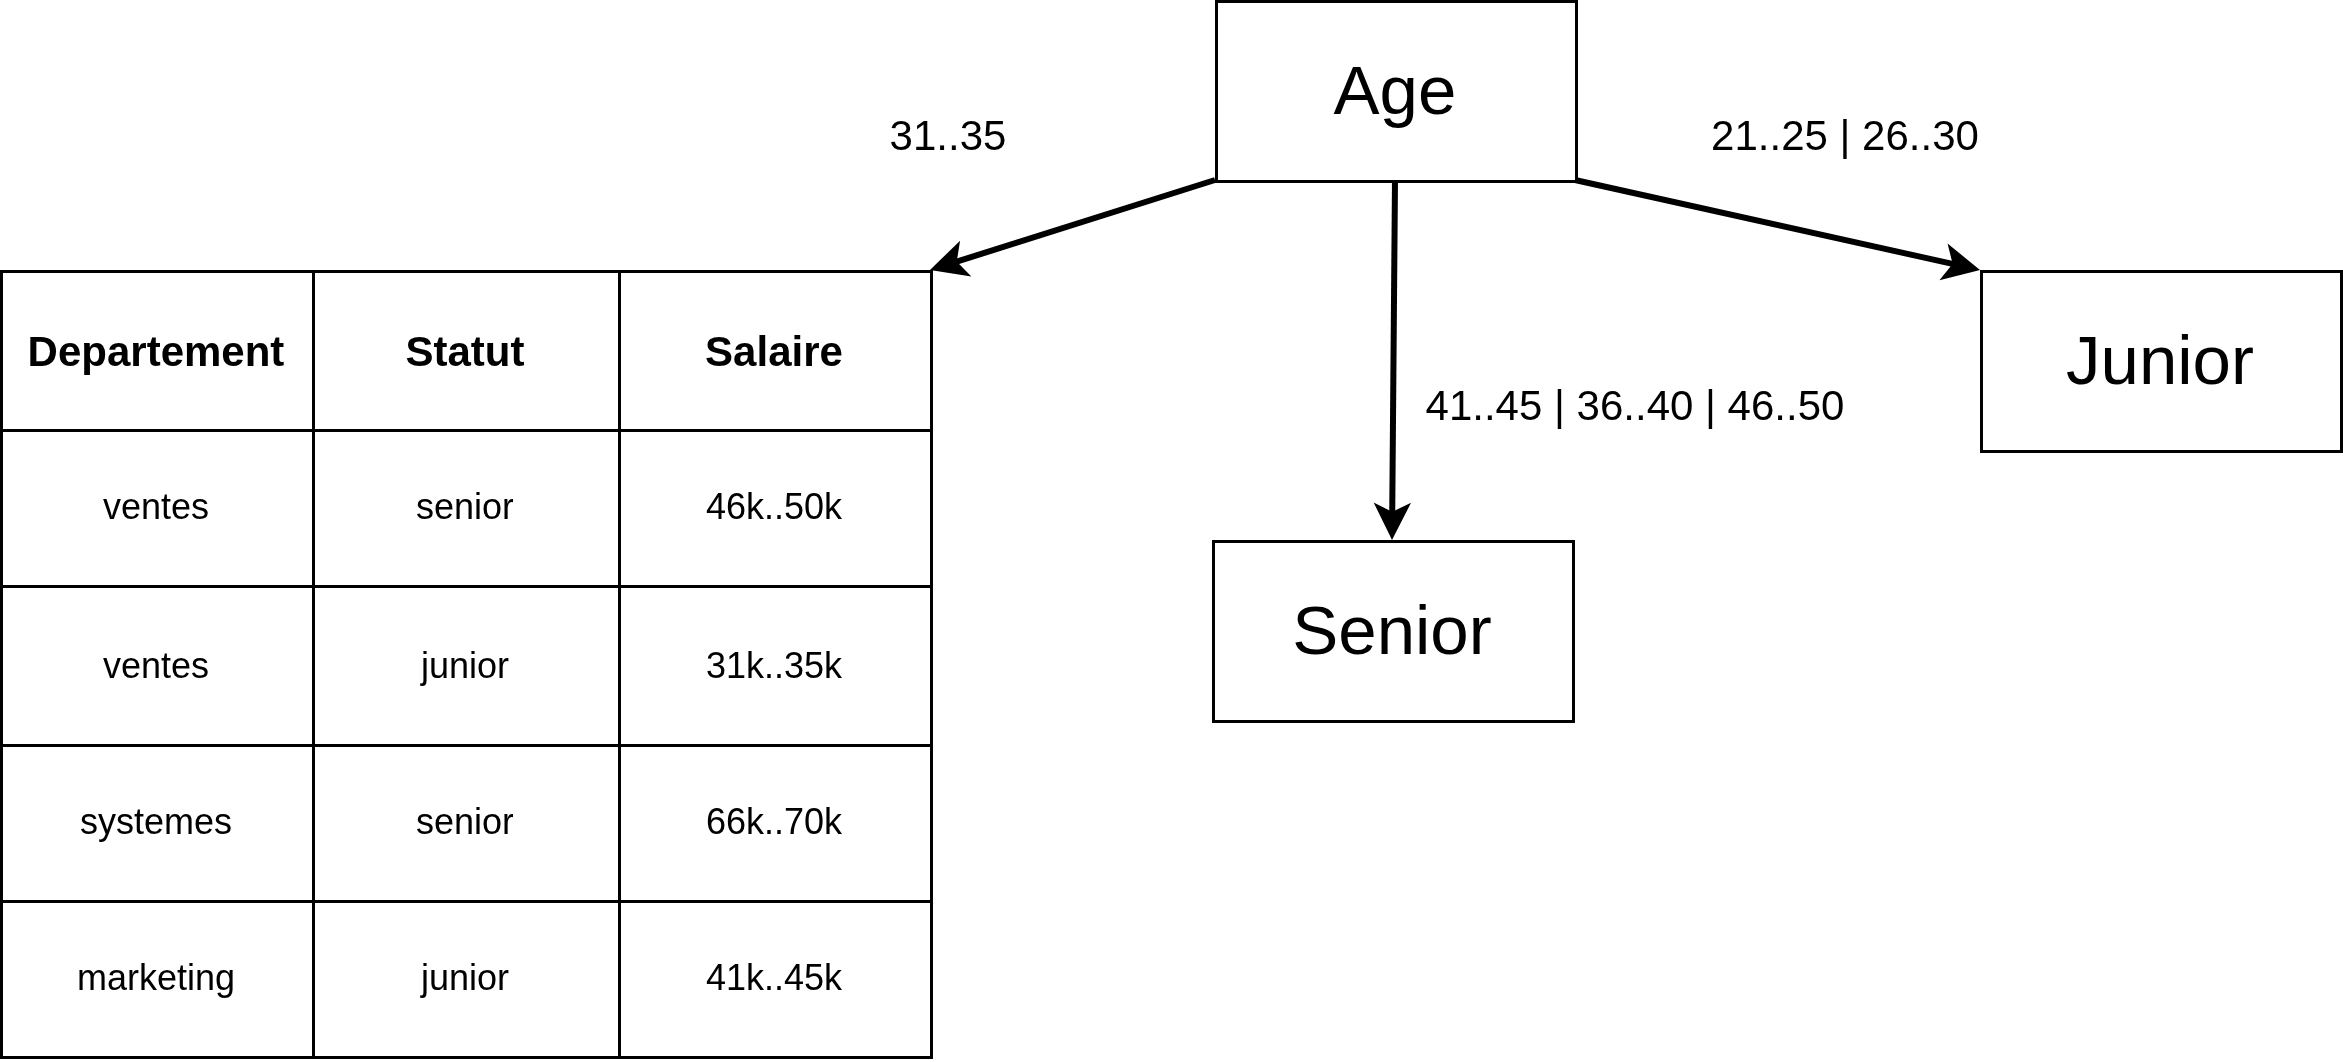
\includegraphics[width=0.75\textwidth]{subTab.png} 
\end{figure}

\newpage
Calcule de l'entropie de class status $H(\text{statut})$ :
\[ - \sum_{i=1}^{C=2} P(y_i) \cdot \log_2\left( P(y_i)\right) = - \left[\underbrace{\dfrac{2}{4} \cdot \log_2\left(\dfrac{2}{4}\right)}_{y_1 = \text{senior}} + \underbrace{\dfrac{2}{4} \cdot \log_2\left(\dfrac{2}{4}\right)}_{y_2  = \text{junior}}\right]  = 1\]

\vspace{0.45cm}

Calcule gain(dep) = $H(\text{statut}) - H(\text{statut} | \text{dep})$ :
\begin{align*}
    H(\text{statut} | \text{dep}) &= \sum_{x\in X} \dfrac{|D_x|}{|D|} \left( - \sum_{i=1} ^{C=2} \dfrac{|D_{x,y}|}{|D_x|} \cdot \log_2 \left( \dfrac{|D_{x,y}|}{|D_x|} \right) \right)\\[0.25cm]
                                  &= \dfrac{2}{4} \cdot \left( - \left[ \textcolor{blue}{\dfrac{1}{2} \cdot \log_2\left (\dfrac{1}{2} \right)} +   \textcolor{red}{\dfrac{1}{2} \cdot \log_2\left (\dfrac{1}{2} \right)} \right]  \right) \quad \text{ventes}\\[0.25cm]
                                  &+ \dfrac{1}{4} \cdot \left( - \left[ \textcolor{red}{\dfrac{1}{1} \cdot \log_2\left (\dfrac{1}{1} \right)} \right]  \right) \quad \text{systemes}\\[0.25cm]
                                  &+ \dfrac{1}{4} \cdot \left( - \left[ \textcolor{blue}{\dfrac{1}{1} \cdot \log_2\left (\dfrac{1}{1} \right)}  \right]  \right) \quad \text{marketing}\\[0.25cm]
                                  & = 0.5
\end{align*}

\[\text{gain(dep)} = H(\text{statut}) - H(\text{statut} | \text{dep}) = 1 - 0.5 = 0.5\]


\vspace{0.45cm}

Calcule gain(salaire) = $H(\text{statut}) - H(\text{statut} | \text{salaire})$ :
\begin{align*}
    H(\text{statut} | \text{salaire}) &= \sum_{x\in X} \dfrac{|D_x|}{|D|} \left( - \sum_{i=1} ^{C=2} \dfrac{|D_{x,y}|}{|D_x|} \cdot \log_2 \left( \dfrac{|D_{x,y}|}{|D_x|} \right) \right)\\[0.25cm]
                                  &= \dfrac{1}{4} \cdot \left( - \left[  \textcolor{red}{\dfrac{1}{1} \cdot \log_2\left (\dfrac{1}{1} \right)} \right]  \right) \quad \text{46k..50k}\\[0.25cm]
                                  &+ \dfrac{1}{4} \cdot \left( - \left[ \textcolor{blue}{\dfrac{1}{1} \cdot \log_2\left (\dfrac{1}{1} \right)}  \right]  \right) \quad \text{31k..35k}\\[0.25cm]
                                  &+ \dfrac{1}{4} \cdot \left( - \left[ \textcolor{red}{\dfrac{1}{1} \cdot \log_2\left (\dfrac{1}{1} \right)}  \right]  \right) \quad \text{66k..70k}\\[0.25cm]
                                  &+ \dfrac{1}{4} \cdot \left( - \left[ \textcolor{blue}{\dfrac{1}{1} \cdot \log_2\left (\dfrac{1}{1} \right)}  \right]  \right) \quad \text{41k..45k}\\[0.25cm]
                                  & = 0
\end{align*}


\vspace{-0.15cm}

\[\text{gain(salaire)} = H(\text{statut}) - H(\text{statut} | \text{salaire}) = 1 - 0 = 1\]

\newpage
Calcule split\_info(dep) :

\vspace{-0.5cm}

\begin{align*}
    \text{split\_info(dep)} &= - \sum_{x \in X} \dfrac{|D_x|}{|D|} \cdot \log_2\left( \dfrac{|D_x|}{|D|} \right) \\[0.25cm]
                            &= - \left( \dfrac{2}{4} \cdot  \log_2\left( \dfrac{2}{4} \right) \quad \text{ventes} \right. \\[0.25cm]
                            &+ \dfrac{1}{4} \cdot  \log_2\left( \dfrac{1}{4} \right) \quad \text{systemes} \\[0.25cm]
                            &+ \left. \dfrac{1}{4} \cdot  \log_2\left( \dfrac{1}{4} \right) \right]\quad \text{marketing} \\[0.25cm]
                            & = 1.5
\end{align*}

\vspace{0.45cm}
Calcule split\_info(salaire) :


\vspace{-0.5cm}

\begin{align*}
    \text{split\_info(salaire)} &= - \sum_{x \in X} \dfrac{|D_x|}{|D|} \cdot \log_2\left( \dfrac{|D_x|}{|D|} \right) \\[0.25cm]
                            &= - \left[ \dfrac{1}{4} \cdot  \log_2\left( \dfrac{1}{4} \right) \quad \text{46k..50k} \right. \\[0.25cm]
                            &+ \dfrac{1}{4} \cdot  \log_2\left( \dfrac{1}{4} \right) \quad \text{31k..35k} \\[0.25cm]
                            &+ \dfrac{1}{4} \cdot  \log_2\left( \dfrac{1}{4} \right) \quad \text{66k..70k} \\[0.25cm]
                            &+ \left .\dfrac{1}{4} \cdot  \log_2\left( \dfrac{1}{4} \right) \right] \quad \text{41k..45k} \\[0.25cm]
                            & = 2
\end{align*}


\vspace{0.75cm}

Calcule gain\_ratio(dep) :
\[ \text{gain\_ratio(dep)} = \dfrac{ \text{gain(dep)} } { \text{split\_info(dep)} } = \dfrac{0.5}{1.5} = 0.333 \]

\vspace{0.25cm}

Calcule gain\_ratio(salaire) :
\[ \text{gain\_ratio(salaire)} = \dfrac{ \text{gain(salaire)} } { \text{split\_info(salaire)} } = \dfrac{1}{2} = 0.5\]

\vspace{0.75cm}

Arbre de decision de la deuxieme iteration :

\vspace{0.15cm}
\begin{figure}[H] 
  \centering 
  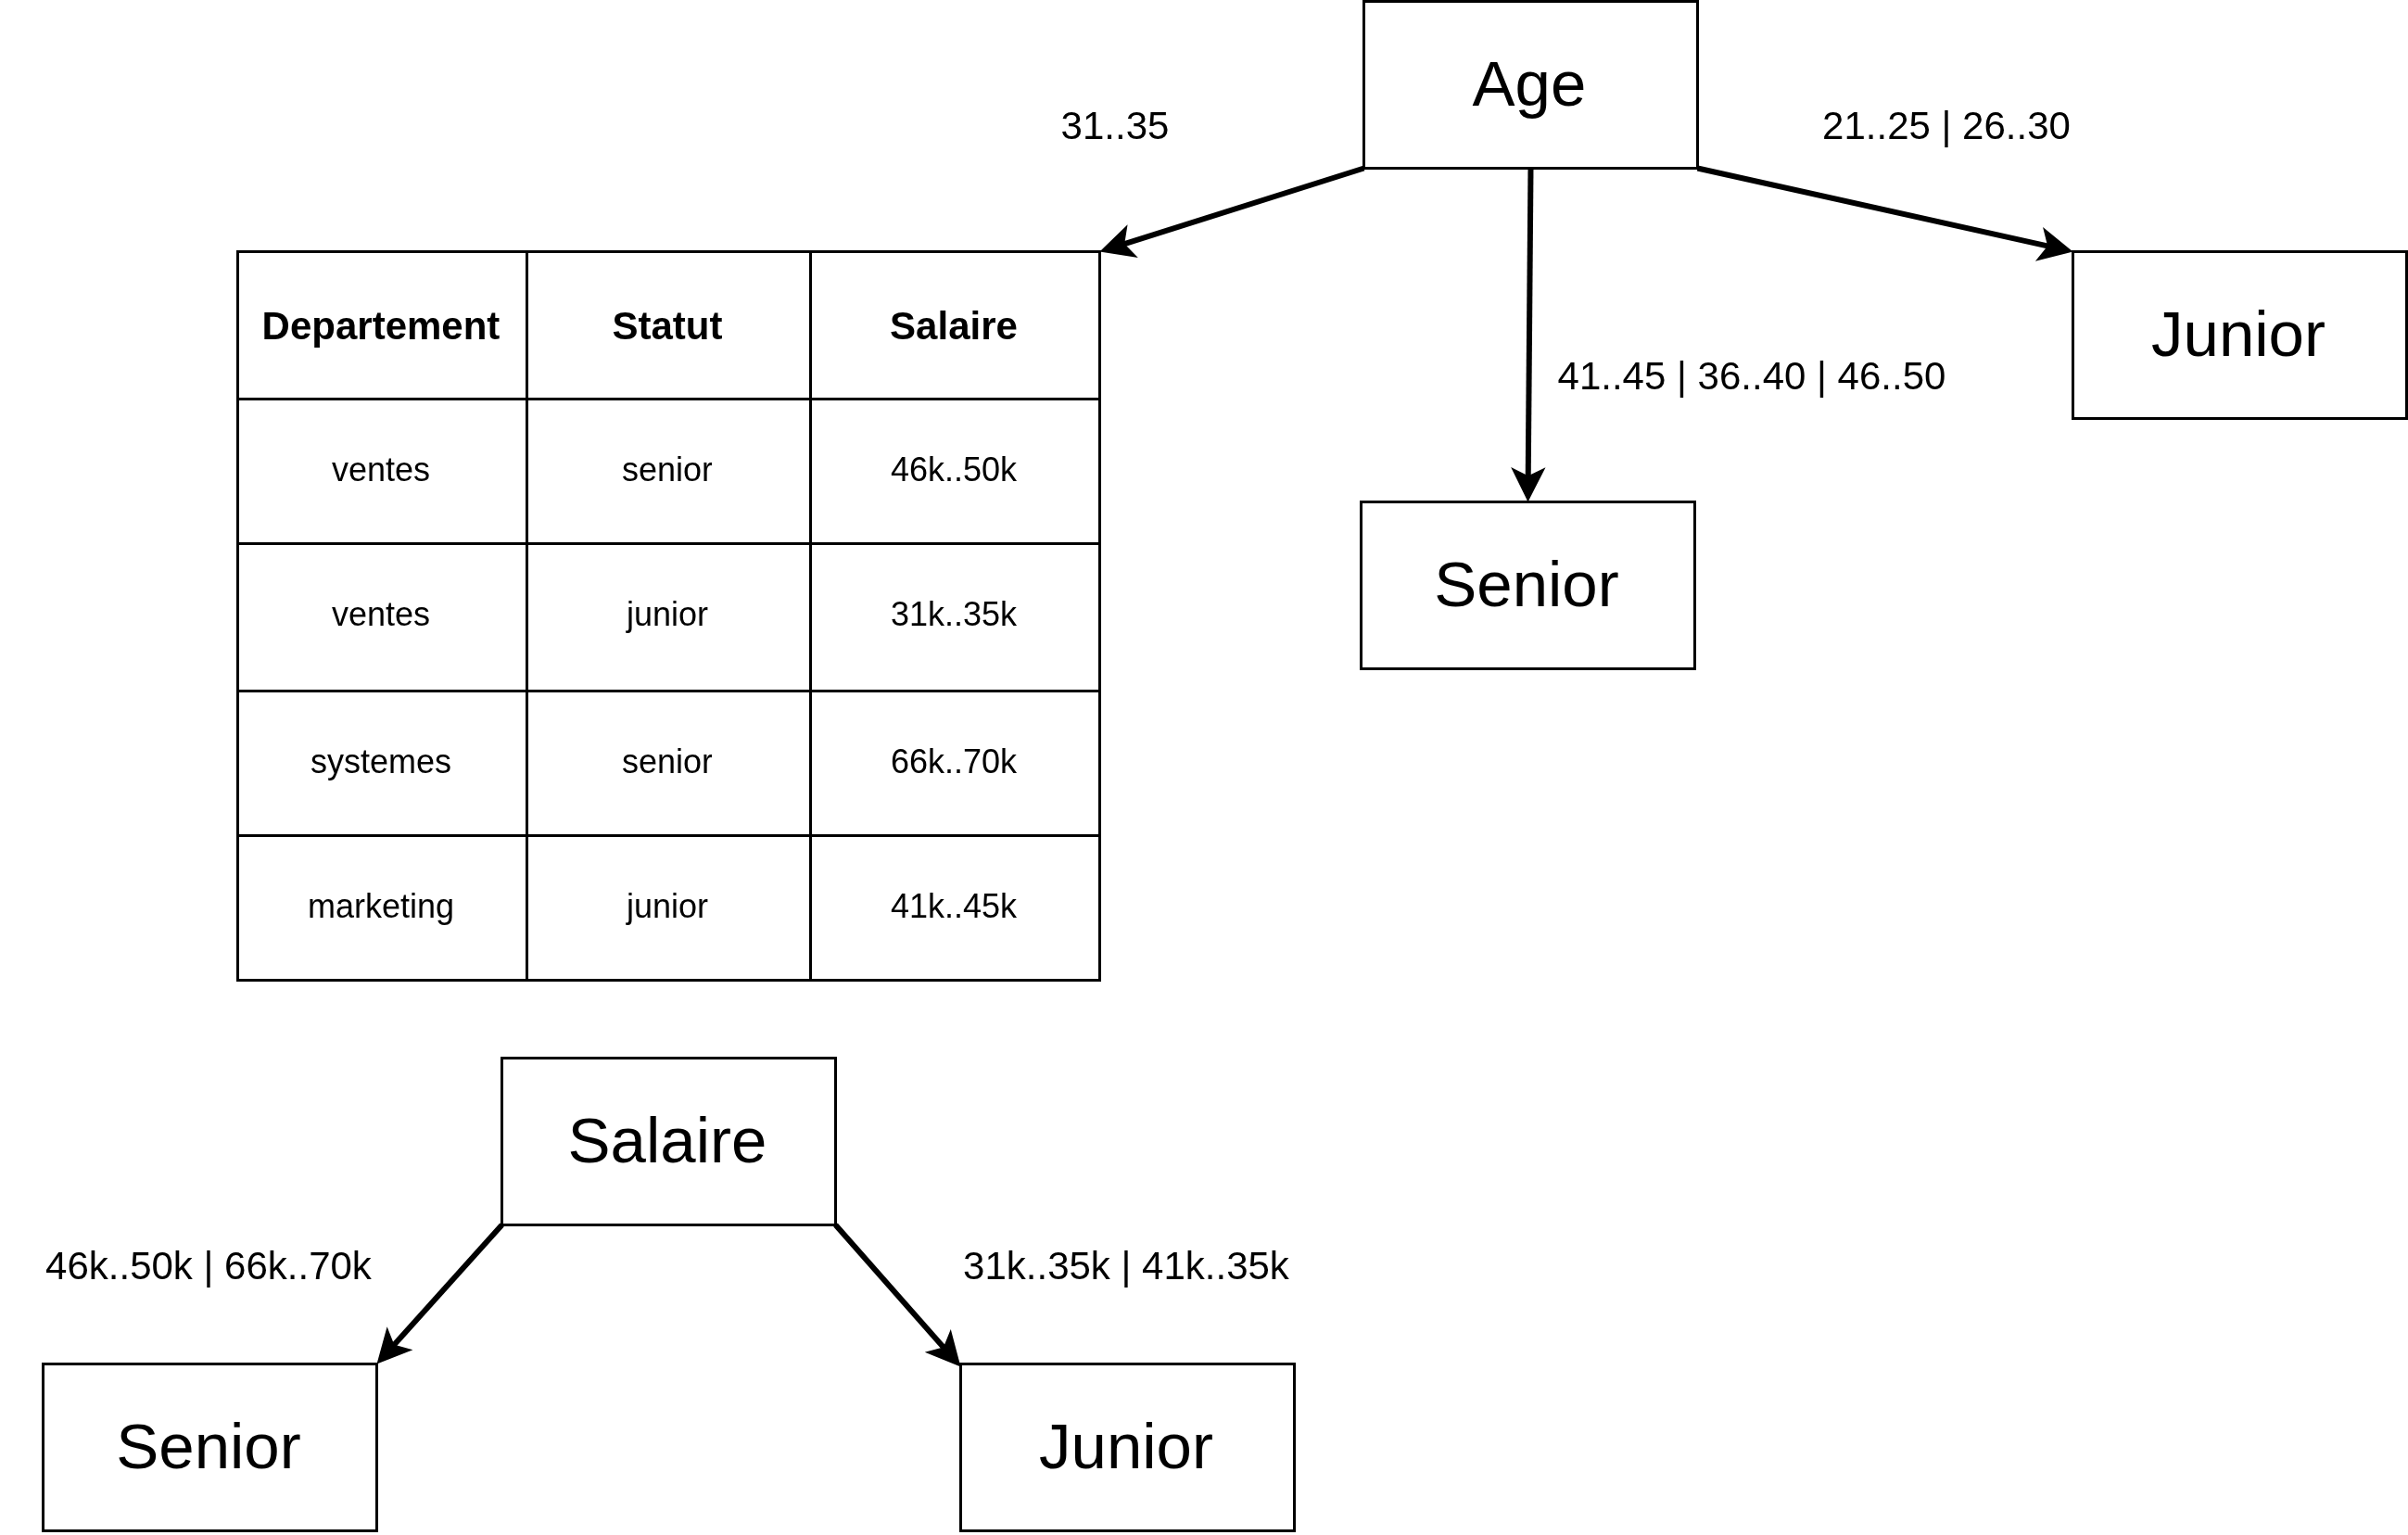
\includegraphics[width=0.65\textwidth]{subTab2.png} 
\end{figure}


\newpage

Comment modifier l’algorithme de l’arbre de décision pour prendre en compte le nombre d’occurrence
de l’instance ?\\[0.25cm]
{\large \textbf{La Solution :}} Au lieu de compter une instance comme 1, on compte sa fréquence lorsqu'on calcule 
les probabilités.

\vspace{0.35cm}
Déduire l’arbre de décision engendré de l’exécution de l’algorithme modifie :

\vspace{0.45cm}
Calcule de l'entropie de class status $H(\text{statut})$ :
\[ - \sum_{i=1}^{C=2} P(y_i) \cdot \log_2\left( P(y_i)\right) = - \left[\underbrace{\dfrac{52}{165} \cdot \log_2\left(\dfrac{52}{165}\right)}_{y_1 = \text{senior}} + \underbrace{\dfrac{113}{165} \cdot \log_2\left(\dfrac{113}{165}\right)}_{y_2  = \text{junior}}\right]  = 0.899\]

\vspace{0.45cm}

Calcule gain(dep) = $H(\text{statut}) - H(\text{statut} | \text{dep})$ :
\begin{align*}
    H(\text{statut} | \text{dep}) &= \sum_{x\in X} \dfrac{|D_x|}{|D|} \left( - \sum_{i=1} ^{C=2} \dfrac{|D_{x,y}|}{|D_x|} \cdot \log_2 \left( \dfrac{|D_{x,y}|}{|D_x|} \right) \right)\\[0.25cm]
                                  &= \dfrac{110}{165} \cdot \left( - \left[ \textcolor{blue}{\dfrac{80}{110} \cdot \log_2\left (\dfrac{80}{110} \right)} +   \textcolor{red}{\dfrac{30}{110} \cdot \log_2\left (\dfrac{30}{110} \right)} \right]  \right) \quad \text{ventes}\\[0.25cm]
                                  &+ \dfrac{31}{165} \cdot \left( - \left[ \textcolor{blue}{\dfrac{23}{31} \cdot \log_2\left (\dfrac{23}{31} \right)} +   \textcolor{red}{\dfrac{8}{31} \cdot \log_2\left (\dfrac{8}{31} \right)} \right]  \right) \quad \text{systemes}\\[0.25cm]
                                  &+ \dfrac{14}{165} \cdot \left( - \left[ \textcolor{blue}{\dfrac{4}{14} \cdot \log_2\left (\dfrac{4}{14} \right)} +   \textcolor{red}{\dfrac{10}{14} \cdot \log_2\left (\dfrac{10}{14} \right)} \right]  \right) \quad \text{marketing}\\[0.25cm]
                                  &+ \dfrac{10}{165} \cdot \left( - \left[ \textcolor{blue}{\dfrac{6}{10} \cdot \log_2\left (\dfrac{6}{10} \right)} +   \textcolor{red}{\dfrac{4}{10} \cdot \log_2\left (\dfrac{4}{10} \right)} \right]  \right) \quad \text{secretariat}\\[0.25cm]
                                  & = 0.850
\end{align*}

\[\text{gain(dep)} = H(\text{statut}) - H(\text{statut} | \text{dep}) = 0.899 - 0.850 = 0.049\]


\vspace{0.45cm}

Calcule gain(age) = $H(\text{statut}) - H(\text{statut} | \text{age})$ :
\begin{align*}
    H(\text{statut} | \text{age}) &= \sum_{x\in X} \dfrac{|D_x|}{|D|} \left( - \sum_{i=1} ^{C=2} \dfrac{|D_{x,y}|}{|D_x|} \cdot \log_2 \left( \dfrac{|D_{x,y}|}{|D_x|} \right) \right)\\[0.25cm]
                                  &= \dfrac{79}{165} \cdot \left( - \left[ \textcolor{blue}{\dfrac{44}{79} \cdot \log_2\left (\dfrac{44}{79} \right)} +   \textcolor{red}{\dfrac{35}{79} \cdot \log_2\left (\dfrac{35}{79} \right)} \right]  \right) \quad \text{31..35}\\[0.25cm]
                                  &+ \dfrac{49}{165} \cdot \left( - \left[ \textcolor{blue}{\dfrac{49}{49} \cdot \log_2\left (\dfrac{49}{49} \right)} \right]  \right) \quad \text{26..30}\\[0.25cm]
                                  &+ \dfrac{20}{165} \cdot \left( - \left[ \textcolor{blue}{\dfrac{20}{20} \cdot \log_2\left (\dfrac{20}{20} \right)}  \right]  \right) \quad \text{21..25}\\[0.25cm]
                                  &+ \dfrac{3}{165} \cdot \left( - \left[ \textcolor{red}{\dfrac{3}{3} \cdot \log_2\left (\dfrac{3}{3} \right)}  \right]  \right) \quad \text{41..45}\\[0.25cm]
                                  &+ \dfrac{10}{165} \cdot \left( - \left[ \textcolor{red}{\dfrac{10}{10} \cdot \log_2\left (\dfrac{10}{10} \right)}  \right]  \right) \quad \text{36..40}\\[0.25cm]
                                  &+ \dfrac{4}{165} \cdot \left( - \left[ \textcolor{red}{\dfrac{4}{4} \cdot \log_2\left (\dfrac{4}{4} \right)}  \right]  \right) \quad \text{46..50}\\[0.25cm]
                                  & = 0.474
\end{align*}


\vspace{-0.15cm}

\[\text{gain(age)} = H(\text{statut}) - H(\text{statut} | \text{age}) = 0.899 - 0.474 = 0.425\]

\vspace{0.45cm}

Calcule gain(salaire) = $H(\text{statut}) - H(\text{statut} | \text{salaire})$ :
\begin{align*}
    H(\text{statut} | \text{salaire}) &= \sum_{x\in X} \dfrac{|D_x|}{|D|} \left( - \sum_{i=1} ^{C=2} \dfrac{|D_{x,y}|}{|D_x|} \cdot \log_2 \left( \dfrac{|D_{x,y}|}{|D_x|} \right) \right)\\[0.25cm]
                                  &= \dfrac{63}{165} \cdot \left( - \left[ \textcolor{blue}{\dfrac{23}{63} \cdot \log_2\left (\dfrac{23}{63} \right)} +   \textcolor{red}{\dfrac{40}{63} \cdot \log_2\left (\dfrac{40}{63} \right)} \right]  \right) \quad \text{46k..50k}\\[0.25cm]
                                  &+ \dfrac{46}{165} \cdot \left( - \left[ \textcolor{blue}{\dfrac{46}{46} \cdot \log_2\left (\dfrac{46}{46} \right)}  \right]  \right) \quad \text{26k..30k}\\[0.25cm]
                                  &+ \dfrac{40}{165} \cdot \left( - \left[ \textcolor{blue}{\dfrac{40}{40} \cdot \log_2\left (\dfrac{40}{40} \right)}  \right]  \right) \quad \text{31k..35k}\\[0.25cm]
                                  &+ \dfrac{8}{165} \cdot \left( - \left[ \textcolor{red}{\dfrac{8}{8} \cdot \log_2\left (\dfrac{8}{8} \right)}  \right]  \right) \quad \text{66k..70k}\\[0.25cm]
                                  &+ \dfrac{4}{165} \cdot \left( - \left[ \textcolor{blue}{\dfrac{4}{4} \cdot \log_2\left (\dfrac{4}{4} \right)}  \right]  \right) \quad \text{41k..45k}\\[0.25cm]
                                  &+ \dfrac{4}{165} \cdot \left( - \left[ \textcolor{red}{\dfrac{4}{4} \cdot \log_2\left (\dfrac{4}{4} \right)}  \right]  \right) \quad \text{36k..40k}\\[0.25cm]
                                  & = 0.361
\end{align*}


\vspace{-0.15cm}

\[\text{gain(salaire)} = H(\text{statut}) - H(\text{statut} | \text{salaire}) = 0.899 - 0.361 = 0.538\]

\vspace{1.15cm}

Calcule split\_info(dep) :


\begin{align*}
    \text{split\_info(dep)} &= - \sum_{x \in X} \dfrac{|D_x|}{|D|} \cdot \log_2\left( \dfrac{|D_x|}{|D|} \right) \\[0.25cm]
                            &= - \left( \dfrac{110}{165} \cdot  \log_2\left( \dfrac{110}{165} \right) \quad \text{ventes} \right. \\[0.25cm]
                            &+ \dfrac{31}{165} \cdot  \log_2\left( \dfrac{31}{165} \right) \quad \text{systemes} \\[0.25cm]
                            &+ \dfrac{14}{165} \cdot  \log_2\left( \dfrac{14}{165} \right) \quad \text{marketing} \\[0.25cm]
                            &+ \left. \dfrac{10}{165} \cdot  \log_2\left( \dfrac{10}{165} \right)\right) \quad \text{secretariat}  \\[0.25cm]
                            & = 1.390
\end{align*}

\newpage

Calcule split\_info(age) :


\begin{align*}
    \text{split\_info(age)} &= - \sum_{x \in X} \dfrac{|D_x|}{|D|} \cdot \log_2\left( \dfrac{|D_x|}{|D|} \right) \\[0.25cm]
                            &= - \left( \dfrac{79}{165} \cdot  \log_2\left( \dfrac{79}{165} \right) \quad \text{31..35} \right. \\[0.25cm]
                            &+ \dfrac{49}{165} \cdot  \log_2\left( \dfrac{49}{165} \right) \quad \text{26..30} \\[0.25cm]
                            &+ \dfrac{20}{165} \cdot  \log_2\left( \dfrac{20}{165} \right) \quad \text{21..25} \\[0.25cm]
                            &+ \dfrac{3}{165} \cdot  \log_2\left( \dfrac{3}{165} \right) \quad \text{41..45} \\[0.25cm]
                            &+ \dfrac{10}{165} \cdot  \log_2\left( \dfrac{10}{165} \right) \quad \text{36..40} \\[0.25cm]
                            &+ \left. \dfrac{4}{165} \cdot  \log_2\left( \dfrac{4}{165} \right)\right) \quad \text{46..50}  \\[0.25cm]
                            & = 1.878
\end{align*}


\vspace{0.45cm}

Calcule split\_info(salaire) :


\begin{align*}
    \text{split\_info(salaire)} &= - \sum_{x \in X} \dfrac{|D_x|}{|D|} \cdot \log_2\left( \dfrac{|D_x|}{|D|} \right) \\[0.25cm]
                            &= - \left( \dfrac{63}{165} \cdot  \log_2\left( \dfrac{63}{165} \right) \quad \text{46k..50k} \right. \\[0.25cm]
                            &+ \dfrac{46}{165} \cdot  \log_2\left( \dfrac{46}{165} \right) \quad \text{26k..30k} \\[0.25cm]
                            &+ \dfrac{40}{165} \cdot  \log_2\left( \dfrac{40}{165} \right) \quad \text{31k..35k} \\[0.25cm]
                            &+ \dfrac{8}{165} \cdot  \log_2\left( \dfrac{8}{165} \right) \quad \text{66k..70k} \\[0.25cm]
                            &+ \dfrac{4}{165} \cdot  \log_2\left( \dfrac{4}{165} \right) \quad \text{41k..45k} \\[0.25cm]
                            &+ \left. \dfrac{4}{165} \cdot  \log_2\left( \dfrac{4}{165} \right)\right) \quad \text{36k..40k}  \\[0.25cm]
                            & = 1.481
\end{align*}

\newpage

Calcule gain\_ratio(dep) :
\[ \text{gain\_ratio(dep)} = \dfrac{ \text{gain(dep)} } { \text{split\_info(dep)} } = \dfrac{0.049}{1.390} = 0.035 \]

\vspace{0.35cm}


Calcule gain\_ratio(age) :
\[ \text{gain\_ratio(age)} = \dfrac{ \text{gain(age)} } { \text{split\_info(age)} } = \dfrac{0.425}{1.878} = 0.226\]

\vspace{0.35cm}

Calcule gain\_ratio(salaire) :
\[ \text{gain\_ratio(salaire)} = \dfrac{ \text{gain(salaire)} } { \text{split\_info(salaire)} } = \dfrac{0.538}{1.481} = 0.363\]

\vspace{1.25cm}

Arbre de decision de la premiere iteration :

\vspace{0.25cm}
\begin{figure}[H] 
  \centering 
  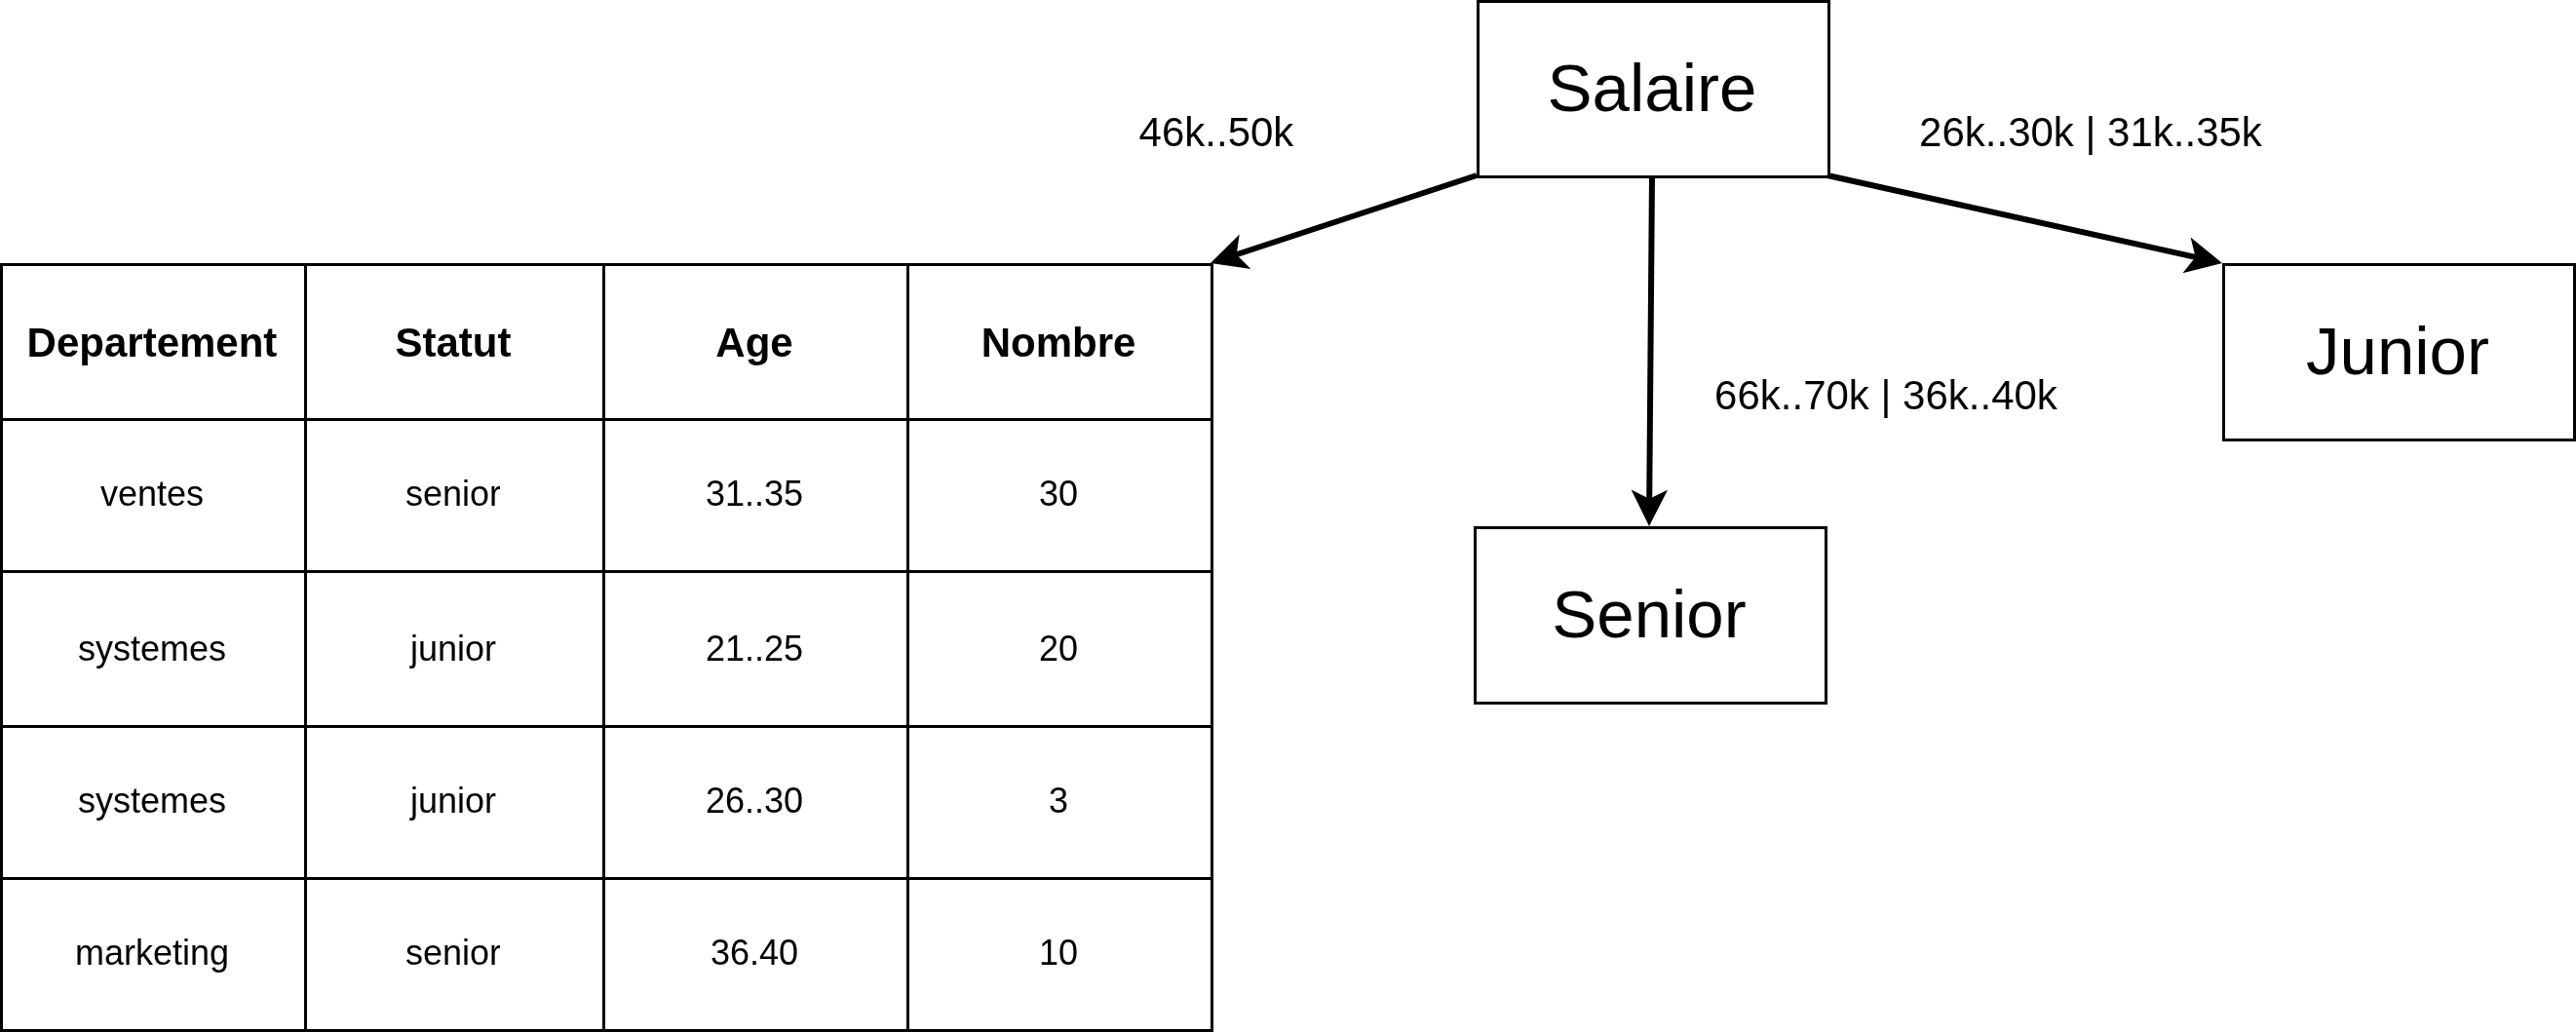
\includegraphics[width=0.75\textwidth]{subTab3.png} 
\end{figure}

\vspace{0.45cm}
Calcule de l'entropie de class status $H(\text{statut})$ :
\[ - \sum_{i=1}^{C=2} P(y_i) \cdot \log_2\left( P(y_i)\right) = - \left[\underbrace{\dfrac{40}{63} \cdot \log_2\left(\dfrac{40}{63}\right)}_{y_1 = \text{senior}} + \underbrace{\dfrac{23}{63} \cdot \log_2\left(\dfrac{23}{63}\right)}_{y_2  = \text{junior}}\right]  = 0.946\]

\vspace{0.45cm}

Calcule gain(dep) = $H(\text{statut}) - H(\text{statut} | \text{dep})$ :
\begin{align*}
    H(\text{statut} | \text{dep}) &= \sum_{x\in X} \dfrac{|D_x|}{|D|} \left( - \sum_{i=1} ^{C=2} \dfrac{|D_{x,y}|}{|D_x|} \cdot \log_2 \left( \dfrac{|D_{x,y}|}{|D_x|} \right) \right)\\[0.25cm]
                                  &= \dfrac{30}{63} \cdot \left( - \left[ \textcolor{red}{\dfrac{30}{30} \cdot \log_2\left (\dfrac{30}{30} \right)} \right]  \right) \quad \text{ventes}\\[0.25cm]
                                  &+ \dfrac{23}{63} \cdot \left( - \left[ \textcolor{blue}{\dfrac{23}{23} \cdot \log_2\left (\dfrac{23}{23} \right)} \right]  \right) \quad \text{systemes}\\[0.25cm]
                                  &+ \dfrac{10}{63} \cdot \left( - \left[ \textcolor{red}{\dfrac{10}{10} \cdot \log_2\left (\dfrac{10}{10} \right)}  \right]  \right) \quad \text{marketing}\\[0.25cm]
                                  & = 0
\end{align*}

\[\text{gain(dep)} = H(\text{statut}) - H(\text{statut} | \text{dep}) = 0.946 - 0 = 0.946\]

\newpage

Calcule gain(age) = $H(\text{statut}) - H(\text{statut} | \text{age})$ :
\begin{align*}
    H(\text{statut} | \text{age}) &= \sum_{x\in X} \dfrac{|D_x|}{|D|} \left( - \sum_{i=1} ^{C=2} \dfrac{|D_{x,y}|}{|D_x|} \cdot \log_2 \left( \dfrac{|D_{x,y}|}{|D_x|} \right) \right)\\[0.25cm]
                                  &= \dfrac{30}{63} \cdot \left( - \left[  \textcolor{red}{\dfrac{30}{30} \cdot \log_2\left (\dfrac{30}{30} \right)} \right]  \right) \quad \text{31..35}\\[0.25cm]
                                  &+ \dfrac{3}{63} \cdot \left( - \left[ \textcolor{blue}{\dfrac{3}{3} \cdot \log_2\left (\dfrac{3}{3} \right)} \right]  \right) \quad \text{26..30}\\[0.25cm]
                                  &+ \dfrac{20}{63} \cdot \left( - \left[ \textcolor{blue}{\dfrac{20}{20} \cdot \log_2\left (\dfrac{20}{20} \right)}  \right]  \right) \quad \text{21..25}\\[0.25cm]
                                  &+ \dfrac{10}{63} \cdot \left( - \left[ \textcolor{red}{\dfrac{10}{10} \cdot \log_2\left (\dfrac{10}{10} \right)}  \right]  \right) \quad \text{36..40}\\[0.25cm]
                                  & = 0
\end{align*}


\vspace{-0.15cm}

\[\text{gain(age)} = H(\text{statut}) - H(\text{statut} | \text{age}) = 0.946 - 0 = 0.946\]

\vspace{0.45cm}




\vspace{0.45cm}
Calcule split\_info(dep) :

\vspace{-0.5cm}

\begin{align*}
    \text{split\_info(dep)} &= - \sum_{x \in X} \dfrac{|D_x|}{|D|} \cdot \log_2\left( \dfrac{|D_x|}{|D|} \right) \\[0.25cm]
                            &= - \left( \dfrac{30}{63} \cdot  \log_2\left( \dfrac{30}{63} \right) \quad \text{ventes} \right. \\[0.25cm]
                            &+ \dfrac{23}{63} \cdot  \log_2\left( \dfrac{23}{63} \right) \quad \text{systemes} \\[0.25cm]
                            &+ \left. \dfrac{10}{63} \cdot  \log_2\left( \dfrac{10}{63} \right) \right]\quad \text{marketing} \\[0.25cm]
                            & = 1.461
\end{align*}

\vspace{0.45cm}
Calcule split\_info(age) :


\begin{align*}
    \text{split\_info(age)} &= - \sum_{x \in X} \dfrac{|D_x|}{|D|} \cdot \log_2\left( \dfrac{|D_x|}{|D|} \right) \\[0.25cm]
                            &= - \left[ \dfrac{30}{63} \cdot  \log_2\left( \dfrac{30}{63} \right) \quad \text{31..35} \right. \\[0.25cm]
                            &+ \dfrac{3}{63} \cdot  \log_2\left( \dfrac{3}{63} \right) \quad \text{26..30} \\[0.25cm]
                            &+ \dfrac{20}{63} \cdot  \log_2\left( \dfrac{20}{63} \right) \quad \text{21..25} \\[0.25cm]
                            &+ \left .\dfrac{10}{63} \cdot  \log_2\left( \dfrac{10}{63} \right) \right] \quad \text{36..40} \\[0.25cm]
                            & = 1.665
\end{align*}

\newpage

Calcule gain\_ratio(dep) :
\[ \text{gain\_ratio(dep)} = \dfrac{ \text{gain(dep)} } { \text{split\_info(dep)} } = \dfrac{0.946}{1.461} = 0.647 \]

\vspace{0.25cm}

Calcule gain\_ratio(age) :
\[ \text{gain\_ratio(age)} = \dfrac{ \text{gain(age)} } { \text{split\_info(age)} } = \dfrac{0.946}{1.665} = 0.568\]

\vspace{1.25cm}

Arbre de decision de la deuxieme iteration :

\vspace{0.25cm}
\begin{figure}[H] 
  \centering 
  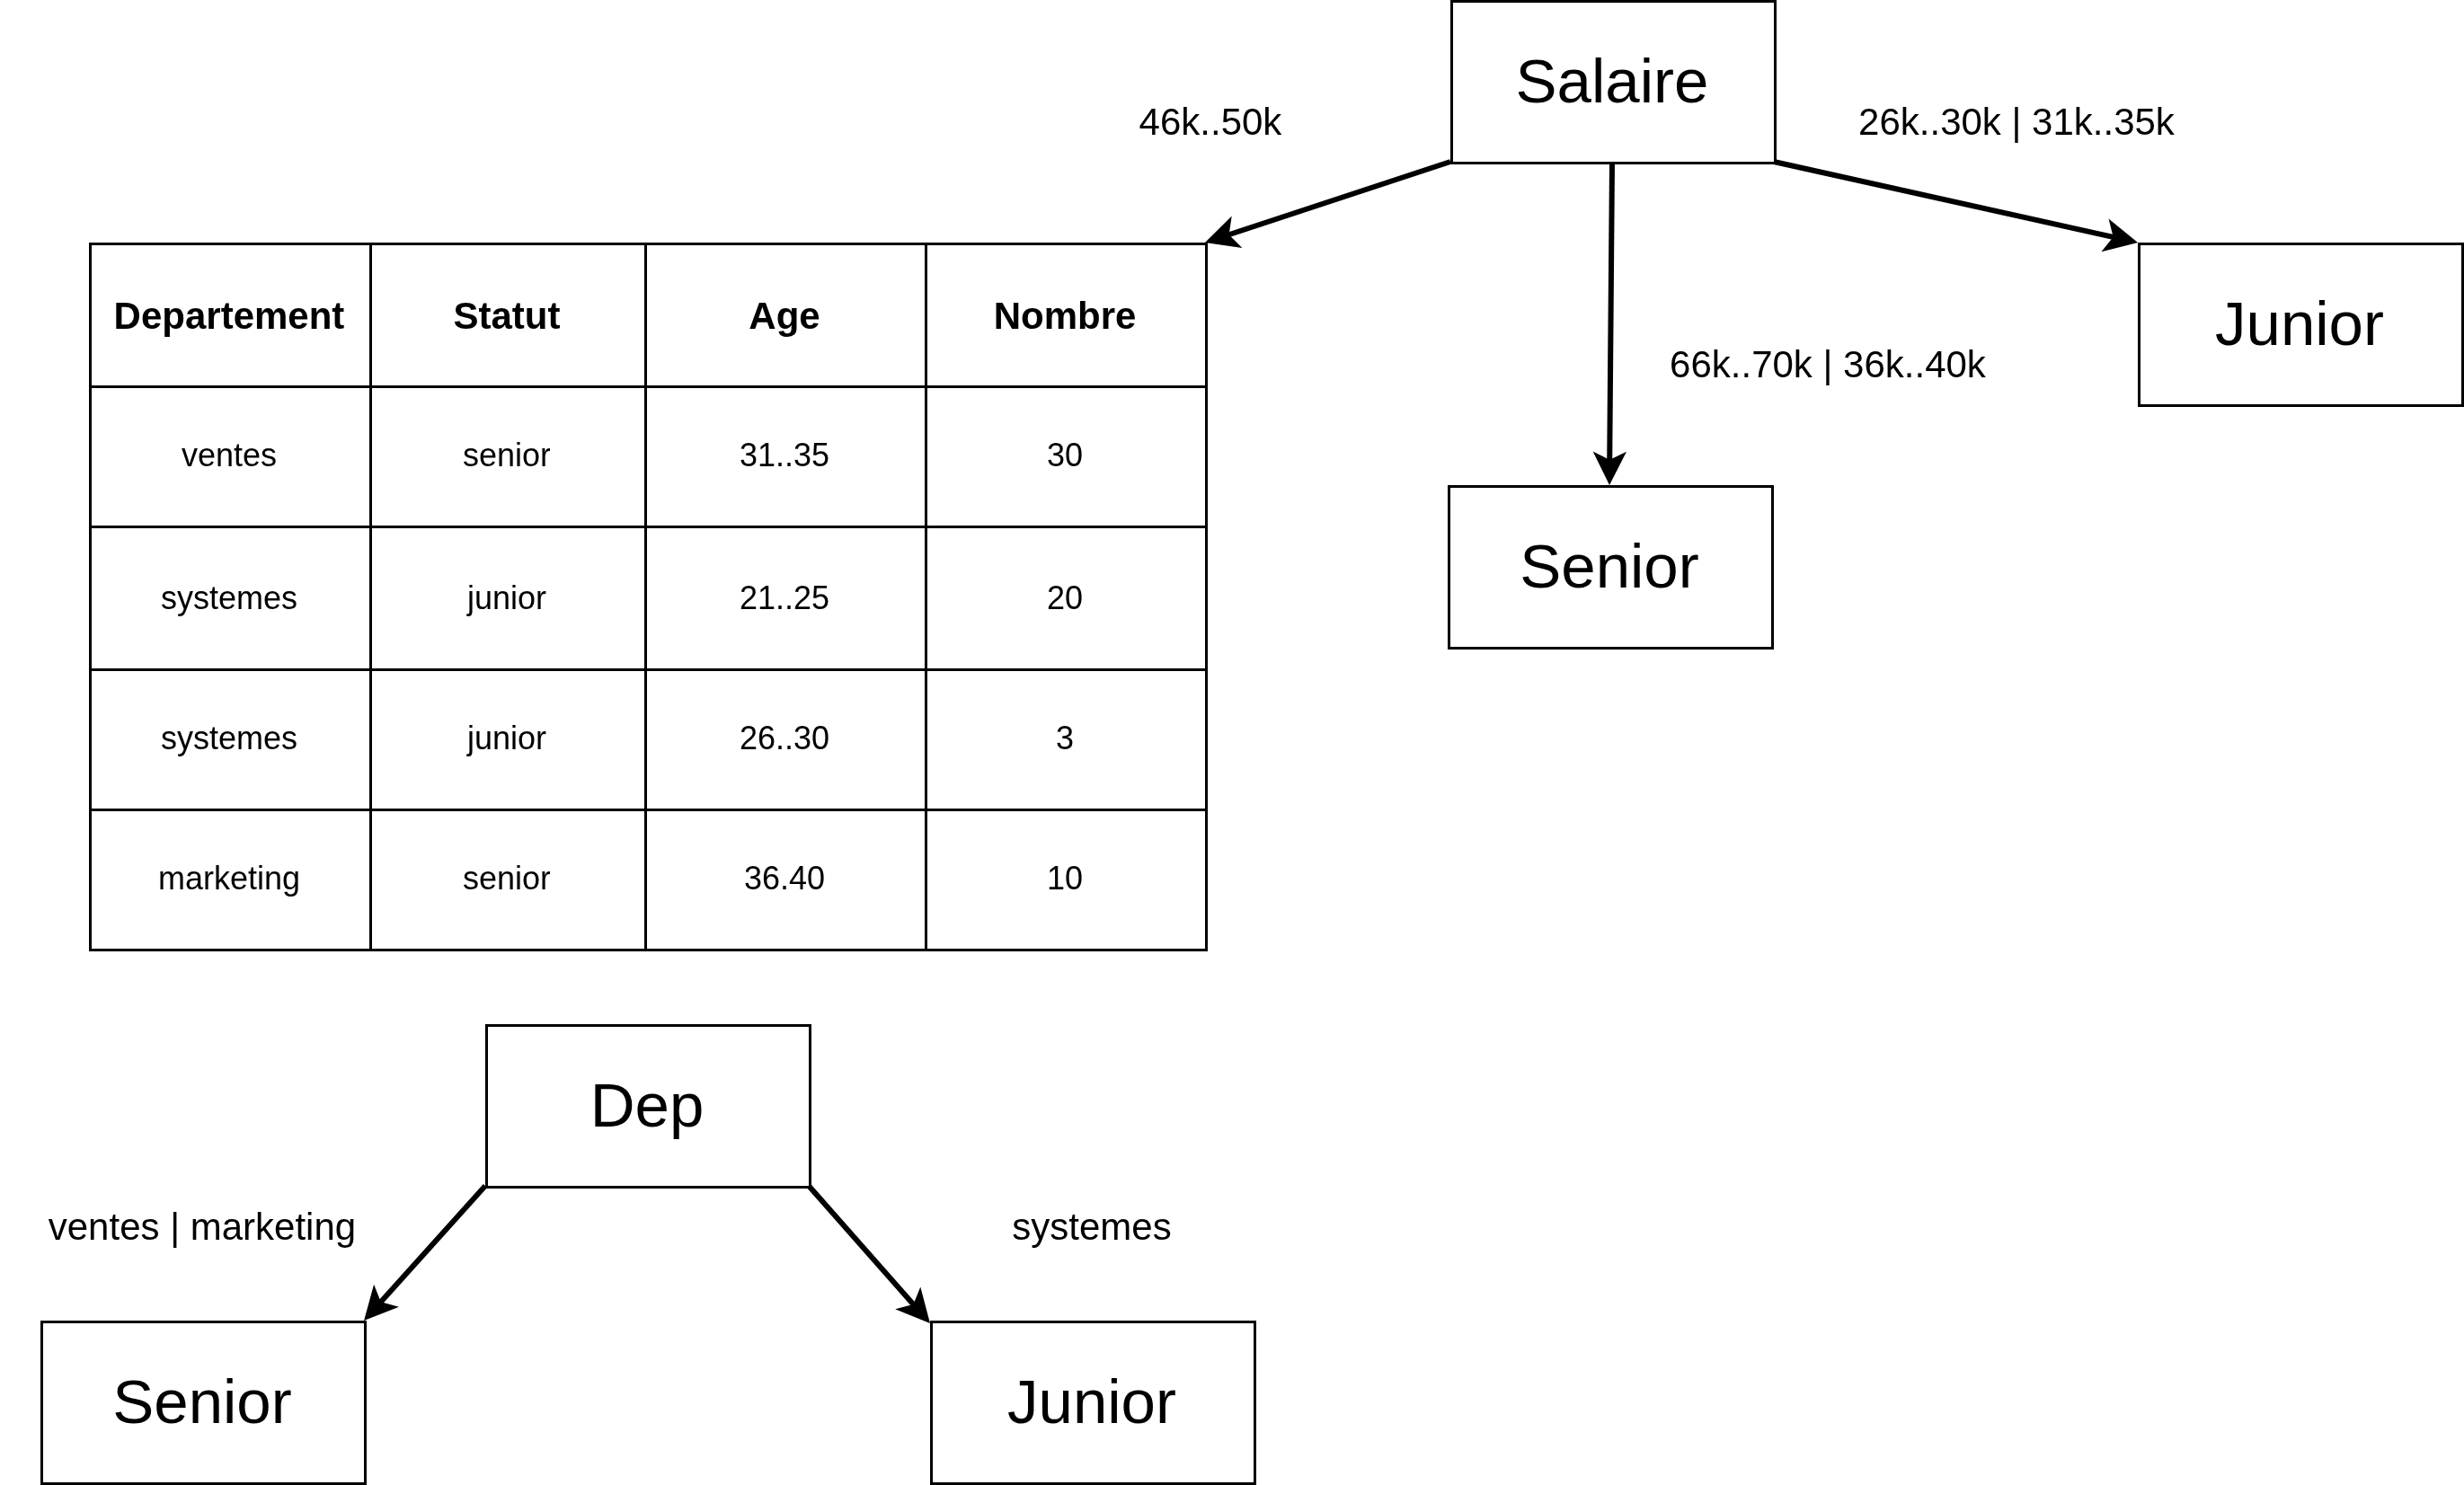
\includegraphics[width=0.65\textwidth]{subTab4.png} 
\end{figure}




\end{document}
